\subsection{Unlocking Signal Strength: Understanding -100 dBm!}

\begin{tcolorbox}[colback=gray!10, colframe=black, title=E4D14`]
What power level does a receiver minimum discernible signal of -100 dBm represent? 

\begin{enumerate}[label=\Alph*.]
    \item 100 microwatts
    \item 0.1 microwatt
    \item 0.001 microwatts
    \item \textbf{0.1 picowatts}
\end{enumerate} \end{tcolorbox}

\subsubsection{Related Concepts and Background}

To answer the above question, we begin by understanding the concept of dBm, which is a unit of power level expressed in decibels relative to 1 milliwatt (mW). The formula to convert dBm to watts (W) is given by:

\[
P (W) = 10^{\frac{P(dBm) - 30}{10}}
\]

In this case, we have a minimum discernible signal (MDS) of -100 dBm. We will apply the conversion formula step-by-step.

\subsubsection{Calculation Steps}

1. Substitute -100 dBm into the formula:
    \[
    P (W) = 10^{\frac{-100 - 30}{10}} = 10^{-13}
    \]

2. Now, to convert the result into a more interpretable form (picoWatts), we note that:
    \[
    1 \, \text{W} = 10^{12} \, \text{pW}
    \]

3. Therefore:
    \[
    10^{-13} \, \text{W} = 10^{-13 + 12} \, \text{pW} = 0.1 \, \text{pW}
    \]

Thus, the minimum discernible signal of -100 dBm corresponds to 0.1 picowatts, which we see corresponds to option D.

\subsubsection{Diagram}

In radio communications, the concept of signal strength can be further understood through a simple diagram showing the relationship of power levels around reference values such as dBm. However, for simplicity, if you would like a visual representation, consider the following illustrative approach:

\begin{center}
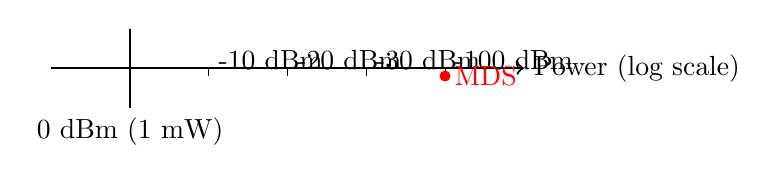
\begin{tikzpicture}
    \draw[->, thick] (-1,0) -- (5,0) node[right] {Power (log scale)};
    \draw[thick] (0,0.5) -- (0,-0.5) node[below] {0 dBm (1 mW)};
    \draw[dashed] (1,-0.1) -- (1,0.1) node[right] {-10 dBm};
    \draw[dashed] (2,-0.1) -- (2,0.1) node[right] {-20 dBm};
    \draw[dashed] (3,-0.1) -- (3,0.1) node[right] {-30 dBm};
    \draw[dashed] (4,-0.1) -- (4,0.1) node[right] {-100 dBm};
    \fill[red] (4,-0.1) circle (2pt) node[right] {MDS};
\end{tikzpicture}
\end{center}
